\chapter{Konzeption des Empfehlungssystems} 
\label{chap:konzeption_des_empfehlungssystems} 

In Kapitel \ref{chap:datenangrundlage_und_trainingsvorbereitung} wurde mit Artefakt A1 eine Trainings- und Evaluationsbasis aus Artikeln und Makros erstellt. 
Anschließend wurde in Kapitel \ref{chap:auswahl_des_modellansatzes} mit LambdaMART ein geeigneter Modellansatz für das Empfehlungssystem ausgewählt. 
Für die Entwicklung des Empfehlungssystems müssen die in Artefakt A1 bereitgestellten Trainings- und Evaluationsbasis und der in Artefakt A2 ausgewählte Modellansatz in eine gemeinsame Architektur überführt werden. 
Das Ziel dieses Kapitels besteht daher in der Entwicklung einer fachlichen Architektur des Empfehlungssystems. Das Ergebnis bildet Artefakt A3. 

\section{Datenobjekte}
\label{sec:datenobjekte}

\subsection{Makroprofil}
\label{sec:makroprofil}

Ein \textit{Makroprofil} wird aus den Artikel-, Makro- und Lexikalvektoren aller einem Makro zugeordneten Trainingsartikel erstellt. Der Artikelvektor liefert hierbei die \textit{technischen Artikeleigenschaften}, 
der Makrovektor die \textit{technischen Makroeigenschaften} und der Lexikalvektor die \textit{technischen Hinweise} aus den Trainingsartikeln.
Enthalten die einem Makro zugeordneten Artikel beispielsweise die Spannungswerte \[ \{380V,\;400V,\;420V\}, \] dann wird jeder Wert ins \textit{Makroprofil} übernommen. 
Dadurch können unterschiedliche Ausprägungen eines Makros berücksichtigt werden, ohne Informationen durch eine Verdichtung auf einen Einzelwert zu verlieren. 
Ein \textit{Makroprofil} beschreibt somit die Menge aller Eigenschaften und Hinweise, die innerhalb eines Makros und dessen zugeordneten Artikeln beobachtet werden können. 

%  Bild 6.1: Aufbau eines Makroprofils

\subsection{Anfrageprofil} 
\label{sec:anfrageprofil} 

Das Anfrageprofil besteht wie das Makroprofil aus den Artikel-, Makro- und Lexikalvektoren, mit dem Unterschied, dass nur ein einzelner Artikel für die Anfrage betrachtet wird. 
In das Anfrageprofil werden die verfügbaren \textit{technischen Artikeleigenschaften}, \textit{technischen Makroeigenschaften} und \textit{technischen Hinweise} der 3 Vektoren übernommen. 
Informationen, welche unmittelbar die Identität des zu empfehlenden Makros zusammenhängen, werden aus dem Anfrageprofil ausgeschlossen. Hierzu zählen die Artikel-Makro-Zuordnung aus dem Artikelvektor sowie 
die Bezeichnung des Makros aus dem Makrovektor. Dadurch wird bei einer Anfrage sichergestellt, dass das Learning-to-Rank-Modell keine direkten Hinweise auf das Zielmakro erhält. 
Anschlussstrukturen und Makrovarianten werden im Anfrageprofil beibehalten, das sie nützliche Informationen für die Unterscheidung von einzelner liefern können.
Die Anfrageprofile werden für alle Teile des Datensplits erstellt, also für Training, Validierung und Test. % WEITER HIER !!

%  Bild 6.2: Aufbau eines Anfrageprofils

\subsection{Anfrage-Kandidat-Paar} 
\label{sec:anfrage_kandidat_paar} 

Ein Anfrage-Kandidat-Paar stellt die Verbindung eines Anfrageprofil mit einem Makroprofil dar. Diese Verbindung ist notwendig, um für das Learning-to-Rank-Modell Lernbeispiele zu erzeugen.
Hierzu wird für jedes vorhanden Makroprofil aus den Trainingsdaten ein Anfrage-Kandidat-Paar mit einem erstelleten Anfrageprofil gebildet.
Stattdessen werden für jedes Anfrage-Kandidat-Paar die in Abschnitt \ref{sec:vergleichsmerkmale} definierten Vergleichsmerkmale berechnet und in einer festen Reihenfolge zu einem Merkmalsvektor zusammengeführt. 
Jede Position dieses Merkmalsvektors besitzt bei allen Anfrage-Kandidat-Paaren dieselbe Bedeutung. 
Besteht der Suchraum beispielsweise aus den Makrokandidaten \(M_1\), \(M_2\) und \(M_3\), werden für eine Anfrage \(q\) die folgenden Paare gebildet: \[ (q,M_1), \qquad (q,M_2), \qquad (q,M_3). \] 
Für jedes Paar entsteht ein eigener Merkmalsvektor: \[ \mathbf{x}_{q,M_1}, \qquad \mathbf{x}_{q,M_2}, \qquad \mathbf{x}_{q,M_3}. \] 
Während des Trainings wird jedem Anfrage-Kandidat-Paar zusätzlich ein Relevanzwert zugeordnet. Dieser wird aus der bekannten Artikel-Makro-Zuordnung abgeleitet und stellt die Zielinformation für LambdaMART dar. 
Bei Validierung, Test und Anwendung berechnet das trainierte Modell für jedes Anfrage-Kandidat-Paar einen Relevanzscore. 
Die Makrokandidaten werden anschließend anhand dieser Relevanzscores in absteigender Reihenfolge sortiert.


\subsection{Vergleichsmerkmale und Merkmalsvektor} 
\label{sec:vergleichsmerkmale} 

Die Makro- und Anfrageprofile können nicht direkt durch das Learning-to-Rank-Modell verarbeitet werden. 
Stattdessen werden aus dem Vergleich dieser Profile numerische Vergleichsmerkmale erzeugt. 
Diese beschreiben die technische Beziehung zwischen einem Anfrageprofil und einem Makroprofil und bilden die Schnittstelle zwischen den Vektoren aus Artefakt A1 und 
dem in Artefakt A2 ausgewählten LambdaMART-Modell. Diese Transformation ist erforderlich, da LambdaMART nur numerische Eingabemerkmale verarbeiten kann. 
Die \textit{technischen Artikel- und Makroeigenschaften} sowie die \textit{technischen Hinweise} müssen deshalb miteinander verglichen werden, 
sodass jede Beziehung zwischen einem Anfrageprofil und einem Makrokandidaten durch einen Zahlenwert beschrieben wird. 
Diese Beziehungen werden anschließend zu einem Merkmalsvektor zusammengeführt, der als Eingabe für das Learning-to-Rank-Modell dient.
Der Merkmalsvektor besitzt dabei immer den gleichen Aufbau. Jede Position im Vektor entspricht einem bestimmten Vergleichsmerkmal, sodass diese später direkt miteinander verglichen werden können.

%  Bild 6.3: Vergleichsmerkmale und Merkmalsvektor









\subsection{Architektur der Datenobjekte}

Die Architektur der in Abschnitt \ref{sec:datenobjekte} eingeführten Datenobjekte ist in Abbildung \ref{fig:datenmodell_empfehlungssystem} dargestellt. 
Die Abbildung zeigt die Überführung der fachlichen Informationen aus den Artikel-, Makro- und Lexikalvektoren in Anfrageprofile, 
Makroprofile, Vergleichsmerkmale und Anfrage-Kandidat-Paare, welche die Eingabe des LambdaMART-Modells bilden.

\begin{figure}[H] 
    \centering 
    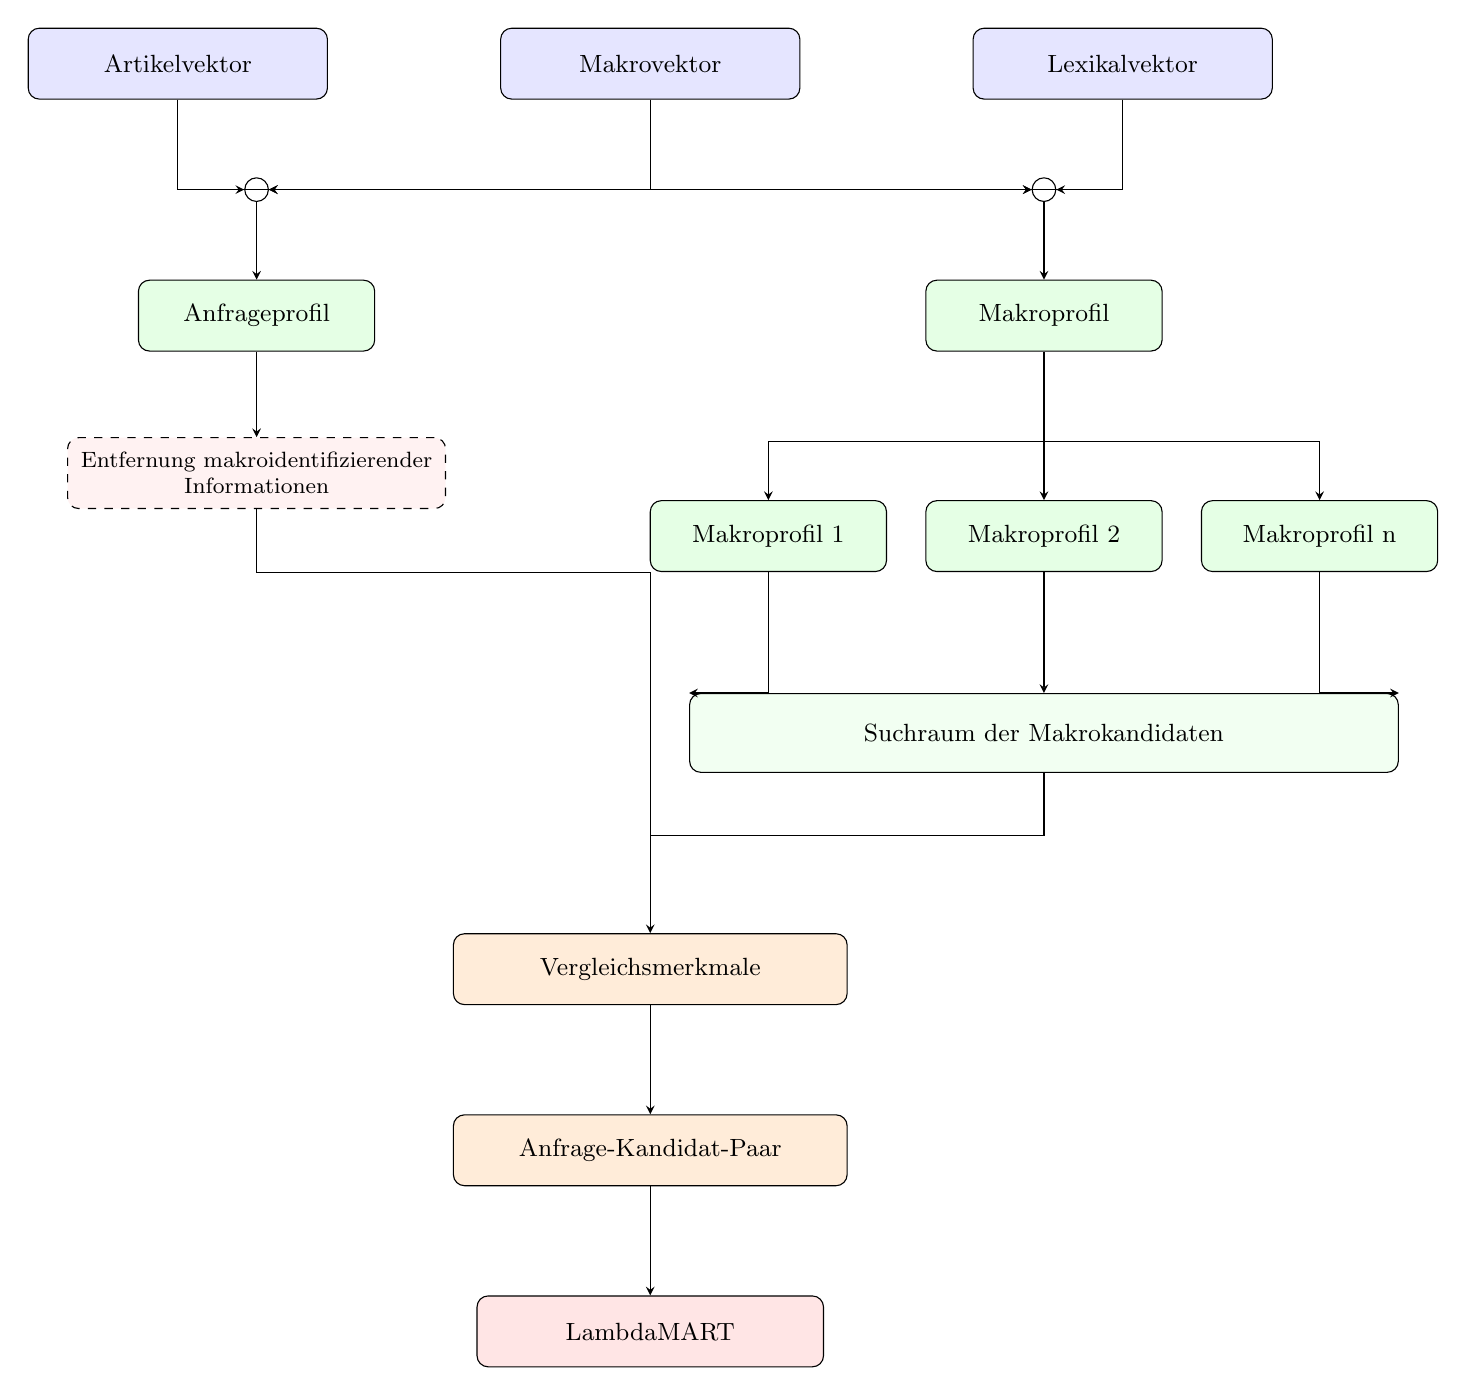
\begin{tikzpicture}[ >=stealth, 
        font=\small, data/.style={ draw, rounded corners, fill=blue!10, minimum width=3.8cm, minimum height=0.9cm, align=center }, 
        profile/.style={ draw, rounded corners, fill=green!10, minimum width=3cm, minimum height=0.9cm, align=center }, 
        filter/.style={ draw, dashed, rounded corners, fill=red!5, minimum width=4.8cm, minimum height=0.9cm, align=center, font=\footnotesize }, 
        feature/.style={ draw, rounded corners, fill=orange!15, minimum width=5.0cm, minimum height=0.9cm, align=center }, 
        model/.style={ draw, rounded corners, fill=red!10, minimum width=4.4cm, minimum height=0.9cm, align=center } ] 
        
        %%%%%%%%%%%%%%%%%%%%%%%%%%%%%%%%%%%%%%%%%%%%%%%%% % Vektoren %%%%%%%%%%%%%%%%%%%%%%%%%%%%%%%%%%%%%%%%%%%%%%%%% 
        
        \node[data] (article) at (-6,8) {Artikelvektor}; 
        \node[data] (macro) at (0,8) {Makrovektor}; 
        \node[data] (lex) at (6,8) {Lexikalvektor}; 

        \node[ draw, circle, fill=white, inner sep=1pt, minimum size=3mm ] (querymerge) at (-5,6.4) {}; 
        \node[ draw, circle, fill=white, inner sep=1pt, minimum size=3mm ] (macromerge) at (5,6.4) {};
        
        %%%%%%%%%%%%%%%%%%%%%%%%%%%%%%%%%%%%%%%%%%%%%%%%% % Anfragezweig %%%%%%%%%%%%%%%%%%%%%%%%%%%%%%%%%%%%%%%%%%%%%%%%% 
        
        \node[profile] (query) at (-5,4.8) {Anfrageprofil}; 
        \node[filter] (filter) at (-5,2.8) { Entfernung makroidentifizierender\\ Informationen }; 
        
        %%%%%%%%%%%%%%%%%%%%%%%%%%%%%%%%%%%%%%%%%%%%%%%%% % Makrozweig %%%%%%%%%%%%%%%%%%%%%%%%%%%%%%%%%%%%%%%%%%%%%%%%% 
        
        \node[profile] (macroprofile) at (5,4.8) {Makroprofil}; 
        
        %%%%%%%%%%%%%%%%%%%%%%%%%%%%%%%%%%%%%%%%%%%%%%%%% % Makroprofile des Suchraums %%%%%%%%%%%%%%%%%%%%%%%%%%%%%%%%%%%%%%%%%%%%%%%%% 
        
        \node[profile] (m1) at (1.5,2.0) {Makroprofil 1}; 
        \node[profile] (m2) at (5.0,2.0) {Makroprofil 2}; 
        \node[profile] (mn) at (8.5,2.0) {Makroprofil n}; 
        
        %%%%%%%%%%%%%%%%%%%%%%%%%%%%%%%%%%%%%%%%%%%%%%%%% % Suchraum %%%%%%%%%%%%%%%%%%%%%%%%%%%%%%%%%%%%%%%%%%%%%%%%% 
        
        \node[ draw, rounded corners, fill=green!5, minimum width=9.0cm, minimum height=1.0cm, align=center ] (searchspace) at (5,-0.5) {Suchraum der Makrokandidaten}; 
        
        %%%%%%%%%%%%%%%%%%%%%%%%%%%%%%%%%%%%%%%%%%%%%%%%% % Vergleich %%%%%%%%%%%%%%%%%%%%%%%%%%%%%%%%%%%%%%%%%%%%%%%%% 
        
        \node[feature] (compare) at (0,-3.5) {Vergleichsmerkmale}; 
        
        %%%%%%%%%%%%%%%%%%%%%%%%%%%%%%%%%%%%%%%%%%%%%%%%% % Anfrage-Kandidat-Paar %%%%%%%%%%%%%%%%%%%%%%%%%%%%%%%%%%%%%%%%%%%%%%%%% 
        
        \node[feature] (pair) at (0,-5.8) {Anfrage-Kandidat-Paar}; 
        
        %%%%%%%%%%%%%%%%%%%%%%%%%%%%%%%%%%%%%%%%%%%%%%%%% % LambdaMART %%%%%%%%%%%%%%%%%%%%%%%%%%%%%%%%%%%%%%%%%%%%%%%%% 
        
        \node[model] (ltr) at (0,-8.1) {LambdaMART}; 
        
        %%%%%%%%%%%%%%%%%%%%%%%%%%%%%%%%%%%%%%%%%%%%%%%%% % Bildung Anfrageprofil %%%%%%%%%%%%%%%%%%%%%%%%%%%%%%%%%%%%%%%%%%%%%%%%% 
        
        \draw[->] (article.south) |- (querymerge); 
        \draw[->] (macro.south) |- (querymerge); 
        \draw[->] (lex.south) |- (querymerge); 
        \draw[->] (querymerge) -- (query.north);

        %%%%%%%%%%%%%%%%%%%%%%%%%%%%%%%%%%%%%%%%%%%%%%%%% % Bildung Makroprofil %%%%%%%%%%%%%%%%%%%%%%%%%%%%%%%%%%%%%%%%%%%%%%%%% 

        \draw[->] (article.south) |- (macromerge); 
        \draw[->] (macro.south) |- (macromerge); 
        \draw[->] (lex.south) |- (macromerge); 
        \draw[->] (macromerge) -- (macroprofile.north);

        \coordinate (macrobranch) at (5,3.2);

        %%%%%%%%%%%%%%%%%%%%%%%%%%%%%%%%%%%%%%%%%%%%%%%%% % Anfrageprofil -> Filter %%%%%%%%%%%%%%%%%%%%%%%%%%%%%%%%%%%%%%%%%%%%%%%%% 

        \draw[->] (query.south) -- (filter.north); 

        %%%%%%%%%%%%%%%%%%%%%%%%%%%%%%%%%%%%%%%%%%%%%%%%% % Makroprofil -> Einzelprofile %%%%%%%%%%%%%%%%%%%%%%%%%%%%%%%%%%%%%%%%%%%%%%%% 

        \draw (macroprofile.south) -- (macrobranch); 
        \draw[->] (macrobranch) -| (m1.north); 
        \draw[->] (macrobranch) -- (m2.north); 
        \draw[->] (macrobranch) -| (mn.north);

        %%%%%%%%%%%%%%%%%%%%%%%%%%%%%%%%%%%%%%%%%%%%%%%%% % Einzelprofile -> Suchraum %%%%%%%%%%%%%%%%%%%%%%%%%%%%%%%%%%%%%%%%%%%%%%%%% 

        \draw[->] (m1.south) -- ++(0,-0.5) |- (searchspace.north west); 
        \draw[->] (m2.south) -- (searchspace.north); 
        \draw[->] (mn.south) -- ++(0,-0.5) |- (searchspace.north east); 

        %%%%%%%%%%%%%%%%%%%%%%%%%%%%%%%%%%%%%%%%%%%%%%%%% % Anfrage + Suchraum -> Vergleich %%%%%%%%%%%%%%%%%%%%%%%%%%%%%%%%%%%%%%%%%%%%%%%%% 

        \coordinate (comparejoin) at (0,-2.0);

        \draw (filter.south) -- ++(0,-0.8) -| (comparejoin); 
        \draw (searchspace.south) -- ++(0,-0.8) -| (comparejoin); 
        \draw[->] (comparejoin) -- (compare.north);

        %%%%%%%%%%%%%%%%%%%%%%%%%%%%%%%%%%%%%%%%%%%%%%%%% % Vergleich -> Paar -> LambdaMART %%%%%%%%%%%%%%%%%%%%%%%%%%%%%%%%%%%%%%%%%%%%%%%%% 

        \draw[->] (compare.south) -- (pair.north); 
        \draw[->] (pair.south) -- (ltr.north); 

    \end{tikzpicture} 
    \caption{ Fachliches Datenmodell des Empfehlungssystems. Artikel-, Makro- und Lexikalvektoren dienen sowohl der Bildung von Anfrageprofilen als auch von Makroprofilen. Aus dem Anfrageprofil werden makroidentifizierende Informationen entfernt. Die Gesamtheit der Makroprofile bildet den Suchraum der Makrokandidaten. Aus dem Vergleich eines Anfrageprofils mit dem Suchraum entstehen Vergleichsmerkmale, welche zu Anfrage-Kandidat-Paaren zusammengeführt und anschließend durch LambdaMART bewertet werden. } 
    \label{fig:datenmodell_empfehlungssystem} 
\end{figure}

\section{Gesamtarchitektur und Datenfluss} 
\label{sec:gesamtarchitektur_und_datenfluss} 

Die Architektur des Empfehlungssystems lässt sich aus der Vision in Abschnitt \ref{sec:vision} ableiten. Ziel des Empfehlungssystems ist es, 
für eine Anfrage geeignete Makros zu identifizieren und diese entsprechend ihrer Relevanz in Form einer sortierten Makro-Liste auszugeben. 
Die Gesamtarchitektur umfasst sowohl den Trainingsprozess als auch den späteren Anwendungsprozess. Beide Prozesse verwenden dieselben Datenstrukturen und dieselbe Berechnung der Vergleichsmerkmale. 
Sie unterscheiden sich jedoch hinsichtlich der Verfügbarkeit der bekannten Artikel-Makro-Zuordnungen und des Zwecks, für den die erzeugten Relevanzwerte verwendet werden. 

\subsection{Überblick über die Gesamtarchitektur}

Abbildung \ref{fig:prozessarchitektur_empfehlungssystem} stellt den Datenfluss des Empfehlungssystems während Training, Validierung, Test und Anwendung dar. 
Die gemeinsame fachliche Grundlage bilden die in Abschnitt \ref{sec:datenobjekte} definierten Makroprofile, Anfrageprofile und Vergleichsmerkmale. 
Der Trainingsprozess erzeugt aus den bekannten Artikel-Makro-Zuordnungen ein LambdaMART-Modell und die Makroprofile des Suchraums. Validierung und Test verwenden diese Ergebnisse zur Bewertung des Modells. 
Im Anwendungsprozess werden das trainierte Modell und die gespeicherten Makroprofile verwendet, um für eine neue Anfrage eine sortierte Makro-Liste zu erzeugen.

\begin{figure}[H] 
    \centering 
    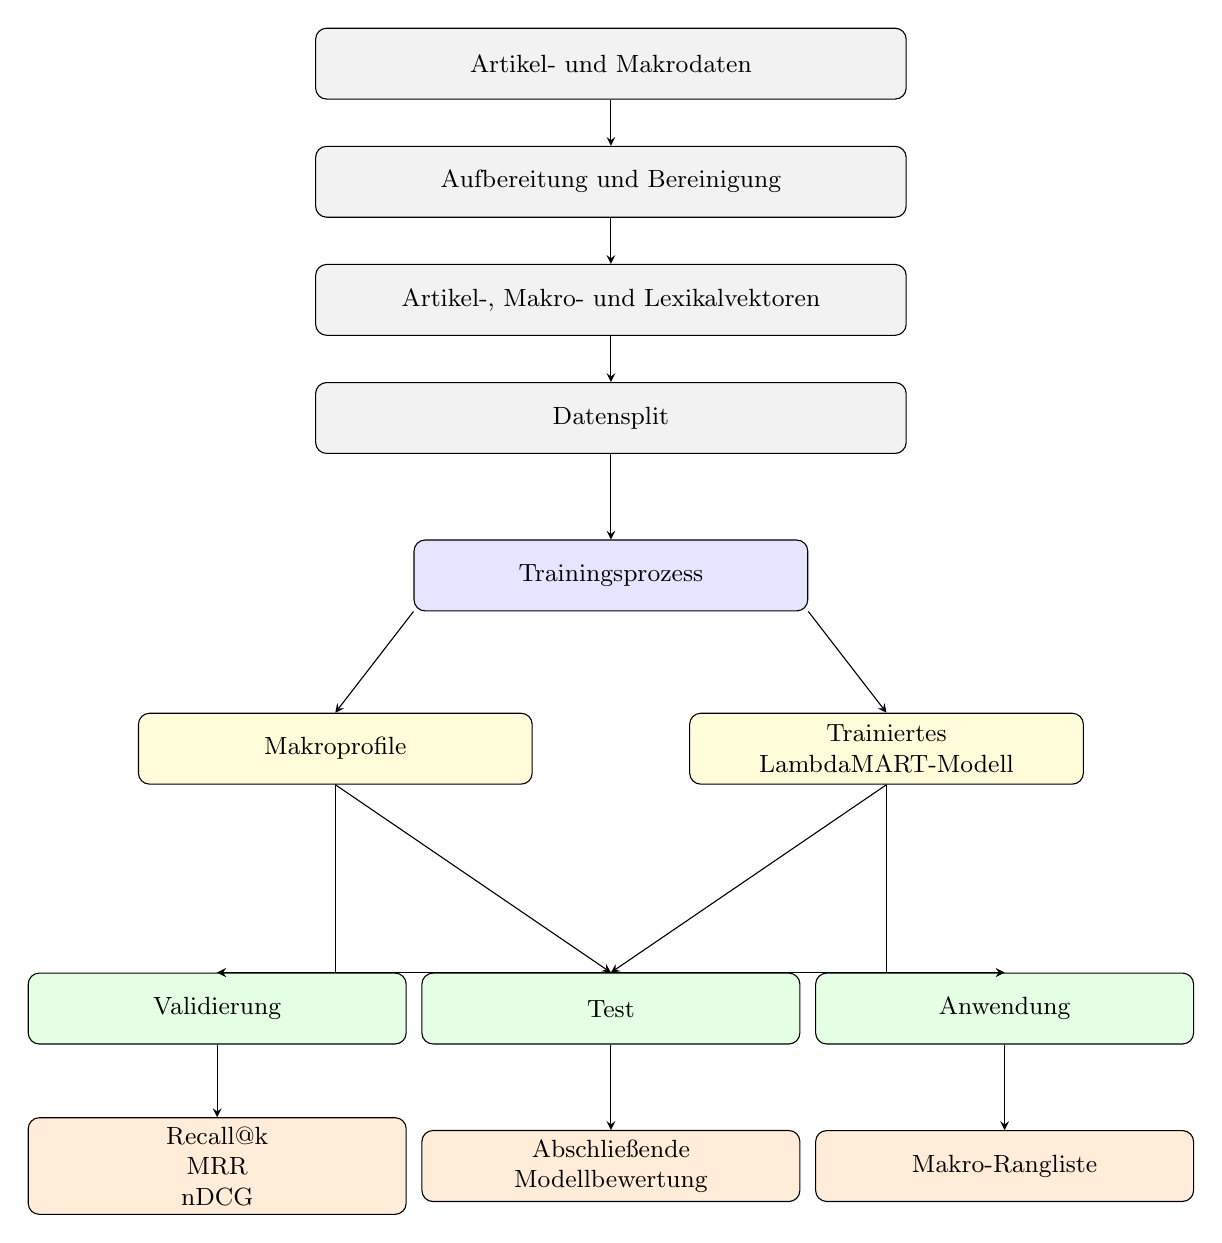
\begin{tikzpicture}[ >=stealth, font=\small, 
        common/.style={ draw, rounded corners, fill=gray!10, minimum width=7.5cm, minimum height=0.9cm, align=center }, 
        train/.style={ draw, rounded corners, fill=blue!10, minimum width=5cm, minimum height=0.9cm, align=center }, 
        artifact/.style={ draw, rounded corners, fill=yellow!15, minimum width=5cm, minimum height=0.9cm, align=center }, 
        process/.style={ draw, rounded corners, fill=green!10, minimum width=4.8cm, minimum height=0.9cm, align=center }, 
        result/.style={ draw, rounded corners, fill=orange!15, minimum width=4.8cm, minimum height=0.9cm, align=center } ] 
        
        %%%%%%%%%%%%%%%%%%%%%%%%%%%%%%%%%%%%%%%%%%%%%%%%% % Datenbasis %%%%%%%%%%%%%%%%%%%%%%%%%%%%%%%%%%%%%%%%%%%%%%%%% 
        
        \node[common] (raw) at (0,10) {Artikel- und Makrodaten}; 
        \node[common] (prep) at (0,8.5) {Aufbereitung und Bereinigung}; 
        \node[common] (vectors) at (0,7.0) {Artikel-, Makro- und Lexikalvektoren}; 
        \node[common] (split) at (0,5.5) {Datensplit}; 
        \draw[->] (raw) -- (prep); 
        \draw[->] (prep) -- (vectors); 
        \draw[->] (vectors) -- (split); 
        
        %%%%%%%%%%%%%%%%%%%%%%%%%%%%%%%%%%%%%%%%%%%%%%%%% % Training %%%%%%%%%%%%%%%%%%%%%%%%%%%%%%%%%%%%%%%%%%%%%%%%% 
        
        \node[train] (training) at (0,3.5) {Trainingsprozess}; 
        \draw[->] (split) -- (training); 
        
        %%%%%%%%%%%%%%%%%%%%%%%%%%%%%%%%%%%%%%%%%%%%%%%%% % Artefakte %%%%%%%%%%%%%%%%%%%%%%%%%%%%%%%%%%%%%%%%%%%%%%%%% 
        
        \node[artifact] (profiles) at (-3.5,1.3) {Makroprofile}; 
        \node[artifact] (ltrmodel) at (3.5,1.3) {Trainiertes\\LambdaMART-Modell}; 
        \draw[->] (training.south west) -- (profiles.north); 
        \draw[->] (training.south east) -- (ltrmodel.north); 
        
        %%%%%%%%%%%%%%%%%%%%%%%%%%%%%%%%%%%%%%%%%%%%%%%%% % Validierung %%%%%%%%%%%%%%%%%%%%%%%%%%%%%%%%%%%%%%%%%%%%%%%%% 
        
        \node[process] (validation) at (-5.0,-2.0) {Validierung}; 
        \node[result] (metrics) at (-5.0,-4.0) {Recall@k\\MRR\\nDCG}; 
        
        %%%%%%%%%%%%%%%%%%%%%%%%%%%%%%%%%%%%%%%%%%%%%%%%% % Test %%%%%%%%%%%%%%%%%%%%%%%%%%%%%%%%%%%%%%%%%%%%%%%%% 
        
        \node[process] (test) at (0,-2.0) {Test}; 
        \node[result] (testranking) at (0,-4.0) {Abschließende\\Modellbewertung}; 
        
        %%%%%%%%%%%%%%%%%%%%%%%%%%%%%%%%%%%%%%%%%%%%%%%%% % Anwendung %%%%%%%%%%%%%%%%%%%%%%%%%%%%%%%%%%%%%%%%%%%%%%%%% 
        
        \node[process] (application) at (5.0,-2.0) {Anwendung}; 
        \node[result] (recommendation) at (5.0,-4.0) {Makro-Rangliste}; 
        
        %%%%%%%%%%%%%%%%%%%%%%%%%%%%%%%%%%%%%%%%%%%%%%%%% % Wiederverwendung %%%%%%%%%%%%%%%%%%%%%%%%%%%%%%%%%%%%%%%%%%%%%%%%% 
        
        \draw[->] (profiles.south) |- (validation.north); 
        \draw[->] (profiles.south) -- (test.north); 
        \draw[->] (profiles.south) |- (application.north); 
        \draw[->] (ltrmodel.south) |- (validation.north); 
        \draw[->] (ltrmodel.south) -- (test.north); 
        \draw[->] (ltrmodel.south) |- (application.north); 
        %%%%%%%%%%%%%%%%%%%%%%%%%%%%%%%%%%%%%%%%%%%%%%%%% % Ergebnisse %%%%%%%%%%%%%%%%%%%%%%%%%%%%%%%%%%%%%%%%%%%%%%%%% 
        \draw[->] (validation) -- (metrics); 
        \draw[->] (test) -- (testranking); 
        \draw[->] (application) -- (recommendation); 
    \end{tikzpicture} 
    \caption{ Prozessarchitektur des Empfehlungssystems. Der Trainingsprozess erzeugt Makroprofile und das trainierte LambdaMART-Modell. 
    Beide Artefakte werden anschließend für Validierung, Test und Anwendung wiederverwendet. } 
    \label{fig:prozessarchitektur_empfehlungssystem} 
\end{figure}

Abbildung \ref{fig:gesamtarchitektur_datenfluss} zeigt die Trennung und die gemeinsamen Bestandteile der Prozesse. Der obere Teil beschreibt die gemeinsame Datenaufbereitung und den Datensplit. 
Im Trainingsprozess werden aus dem Trainingssplit die Makroprofile aufgebaut und die Anfrage-Kandidat-Paare für das Lernen des LambdaMART-Modells erzeugt. 
Validierungs- und Testanfragen werden gegen dieselben Makroprofile verglichen. Die daraus erzeugten Ranglisten werden mit den bekannten Artikel-Makro-Zuordnungen bewertet. 
Nur die Validierung darf zur Auswahl oder Anpassung der Modellkonfiguration verwendet werden. Die Testergebnisse dienen ausschließlich der abschließenden Bewertung. 
Der untere Teil zeigt den Anwendungsprozess. Eine neue Anfrage wird in ein Anfrageprofil überführt und mit den gespeicherten Makroprofilen verglichen. 
Die daraus erzeugten Anfrage-Kandidat-Paare werden vom trainierten LambdaMART-Modell bewertet. Als Ergebnis entsteht eine nach Relevanz sortierte Makro-Liste. 
Da für die neue Anfrage keine bekannte Makrozuordnung vorliegt, endet der reguläre Anwendungsprozess mit der Ausgabe der Rangliste.


\subsection{Trainingsprozess} 

Der Trainingsprozess dient dazu, aus den bekannten Artikel-Makro-Zuordnungen ein LambdaMART-Modell zu erzeugen. Hierzu werden die aufbereiteten und bereinigten Daten zunächst in Trainings-, 
Validierungs- und Testdaten aufgeteilt. Der Datensplit erfolgt vor dem Aufbau der Makroprofile, sodass keine Informationen aus den Validierungs- oder Testdaten in deren Bildung einfließen. 
Die Makroprofile werden ausschließlich aus den Daten des Trainingssplits nach der in Abschnitt \ref{sec:makroprofil} beschriebenen Vorgehensweise gebildet. 
Zusätzlich wird jeder Trainingsartikel als Trainingsanfrage betrachtet und in ein Anfrageprofil überführt. Für jedes Anfrageprofil wird mit jedem verfügbaren Makrokandidaten ein Anfrage-Kandidat-Paar gebildet. 
Hierzu werden die in Abschnitt \ref{sec:vergleichsmerkmale} definierten Vergleichsmerkmale berechnet und in einer festen Reihenfolge zu einem Merkmalsvektor zusammengeführt. 
Die bekannte Artikel-Makro-Zuordnung wird dabei nicht als Vergleichsmerkmal verwendet. Sie dient ausschließlich zur Festlegung des Relevanzwertes, der die Zielinformation des jeweiligen Anfrage-Kandidat-Paares darstellt. 
Die Merkmalsvektoren und die zugehörigen Relevanzwerte bilden gemeinsam die Trainingsgrundlage von LambdaMART. 
Das Modell lernt daraus, welche Vergleichsmerkmale und Merkmalskombinationen für die Rangfolge der Makrokandidaten relevant sind. 
Das Ergebnis des Trainingsprozesses besteht aus dem trainierten LambdaMART-Modell, der festgelegten Struktur der Vergleichsmerkmale und den aus dem Trainingssplit erzeugten Makroprofilen. 
Diese Ergebnisse werden in Validierung, Test und Anwendung wiederverwendet.


\subsection{Validierungs- und Testprozess} 

Für jeden Validierungs- und Testartikel wird ein Anfrageprofil nach Abschnitt \ref{sec:anfrageprofil} erzeugt. 
Die bekannte Artikel-Makro-Zuordnung bleibt außerhalb des Anfrageprofils erhalten und wird nicht als Eingabe des Modells verwendet. 
Das Anfrageprofil wird mit allen aus dem Trainingssplit erzeugten Makroprofilen verglichen. 
Die daraus gebildeten Anfrage-Kandidat-Paare besitzen dieselbe Struktur und Reihenfolge der Vergleichsmerkmale wie die Paare des Trainingsprozesses. 
Das trainierte LambdaMART-Modell berechnet für jedes Paar einen Relevanzscore. Durch deren absteigende Sortierung entsteht die Makro-Rangliste. 
Validierung und Test unterscheiden sich nicht in der technischen Verarbeitung, sondern in ihrem Verwendungszweck. 
Die Validierungsergebnisse dürfen zur Auswahl der Modellparameter und Modellvariante verwendet werden. 
Die Testdaten werden erst nach Abschluss dieser Auswahl eingesetzt und dienen ausschließlich der abschließenden Bewertung. 
Hierzu wird die erzeugte Rangliste mit der außerhalb des Anfrageprofils gespeicherten Artikel-Makro-Zuordnung verglichen. 
Die Bewertung erfolgt anhand der in Abschnitt \ref{sec:evaluationsmetriken} beschriebenen Metriken Recall@k, MRR und nDCG.


\subsection{Anwendungsprozess} 

Der Anwendungsprozess beginnt mit einer neuen Anfrage, für die keine Artikel-Makro-Zuordnung bekannt ist. Aus den verfügbaren Informationen wird das in Abschnitt \ref{sec:anfrageprofil} definierte Anfrageprofil erzeugt. 
Das Anfrageprofil wird mit den gespeicherten Makroprofilen aller verfügbaren Makrokandidaten verglichen. 
Für jeden Makrokandidaten werden die in Abschnitt \ref{sec:vergleichsmerkmale} definierten Vergleichsmerkmale in derselben Reihenfolge wie während des Trainings berechnet und zu einem Anfrage-Kandidat-Paar zusammengeführt. 
Das trainierte LambdaMART-Modell berechnet für jedes Anfrage-Kandidat-Paar einen Relevanzscore. Die Makrokandidaten werden anhand dieser Werte in absteigender Reihenfolge sortiert. 
Das Ergebnis ist eine Makro-Liste, in der die nach Bewertung des Modells am besten zur Anfrage passenden Makrokandidaten an den oberen Rangpositionen stehen. 
Da keine bekannte Artikel-Makro-Zuordnung vorliegt, kann die Rangliste im regulären Anwendungsprozess nicht unmittelbar bewertet werden. 
Eine Berechnung der Evaluationsmetriken ist erst möglich, wenn nachträglich eine fachlich geprüfte Artikel-Makro-Zuordnung oder eine fachliche Relevanzbewertung der empfohlenen Makros vorliegt.

\subsection{Gemeinsamkeiten, Unterschiede und Grenzen} 

Training, Validierung, Test und Anwendung verwenden dieselben Makroprofile sowie dieselbe Struktur und Reihenfolge der Vergleichsmerkmale. 
Dadurch entspricht die Eingabestruktur bei der späteren Anwendung der Struktur, auf deren Grundlage LambdaMART trainiert wurde. 
Die Prozesse unterscheiden sich hauptsächlich in der Verwendung der Artikel-Makro-Zuordnung. Im Training wird sie zur Erzeugung der Relevanzwerte verwendet. 
Bei Validierung und Test dient sie ausschließlich zur Bewertung der Rangliste. Im Anwendungsprozess ist sie unbekannt. Die Makroprofile werden ausschließlich aus dem Trainingssplit erzeugt. 
Validierungs-, Test- und Anfrageartikel dürfen nicht in diese Profile einfließen. Dadurch wird verhindert, dass Informationen aus den zu bewertenden Daten in den Suchraum übernommen werden. 
Das Empfehlungssystem ist auf die vorhandenen Makroprofile und Vergleichsmerkmale begrenzt. Ein Makro ohne Makroprofil gehört nicht zum Suchraum und kann nicht empfohlen werden. 
Ebenso können nur Eigenschaften berücksichtigt werden, die durch die vorhandenen Vektoren und Vergleichsmerkmale abgebildet sind. 

Tabelle \ref{tab:vergleich_train_validierung_test_anwendung} fasst die Verwendung der Datenobjekte in den einzelnen Prozessen zusammen.

\begin{table}[H] 
    \centering 
    \caption{Gemeinsamkeiten und Unterschiede zwischen Training, Validierung, Test und Anwendung} 
    \label{tab:vergleich_train_validierung_test_anwendung} 
    \renewcommand{\arraystretch}{1.25} \begin{tabular}{p{3.1cm}p{3.0cm}p{3.0cm}p{3.0cm}} 
        \hline \textbf{Aspekt} & \textbf{Training} & \textbf{Validierung und Test} & \textbf{Anwendung} \\ 
        \hline Anfrageprofil & aus Trainingsartikeln & aus Validierungs- beziehungsweise Testartikeln & aus einer neuen Anfrage \\ 
        Makroprofile & aus dem Trainingssplit erzeugt & aus dem Training übernommen & aus dem Training übernommen \\ 
        Vergleichsmerkmale & werden für jedes Anfrage-Kandidat-Paar berechnet & werden in derselben Form berechnet & werden in derselben Form berechnet \\ 
        Artikel-Makro-Zuordnung & zur Festlegung der Relevanzwerte der Anfrage-Kandidat-Paare verwendet & ausschließlich zur Bewertung der Ranglisten verwendet & nicht vorhanden \\
        LambdaMART & lernt die Bewertung der Vergleichsmerkmale & berechnet Relevanzscore & berechnet Relevanzscore \\
        Ergebnis & trainiertes Modell, Makroprofile und Struktur der Vergleichsmerkmale & Bewertungsmetriken und Ranglisten & sortierte Makro-Liste \\
        Rückwirkung & Modellparameter werden angepasst & nur Validierung darf Modellentscheidungen beeinflussen & keine Modellanpassung während der Anfrage \\ 
        \hline 
    \end{tabular} 
\end{table}


% \subsubsection{Anfrage-Kandidat-Paar} 

% Die Gesamtheit aller Vergleichsmerkmale eines Anfrageprofils und eines Makroprofils wird als Anfrage-Kandidat-Paar bezeichnet. 
% Ein Anfrage-Kandidat-Paar besteht somit nicht aus den ursprünglichen Profilen selbst, sondern aus den aus ihnen berechneten Vergleichsmerkmalen. 
% Für jedes Makroprofil wird ein eigenes Anfrage-Kandidat-Paar erzeugt. LambdaMART bewertet diese Anfrage-Kandidat-Paare anhand der enthaltenen Vergleichsmerkmale und berechnet daraus einen Relevanzscore.
% Für jeden Makrokandidaten wird ein eigenes Anfrage-Kandidat-Paar erzeugt. 
% LambdaMART bewertet diese Paare anhand der enthaltenen Vergleichsmerkmale und berechnet für jeden Kandidaten einen Relevanzscore. 
% Die resultierenden Scores bilden die Grundlage für die Sortierung der Makrokandidaten und somit für die finale Empfehlung.


\section{Kapitelergebnis} 

Ziel dieses Kapitels war die Entwicklung einer Architektur für das Empfehlungssystem auf Grundlage der in Artefakt A1 bereitgestellten Trainingsbasis und des in Artefakt A2 ausgewählten LambdaMART-Verfahrens. 
Hierzu wurden die Komponenten, Datenflüsse und Datenstrukturen des Systems definiert. Besonderes Augenmerk lag auf der Trennung von Anfrageprofilen, Makroprofilen und den daraus gebildeten Vergleichsmerkmalen, 
welche die eigentliche Eingabe des Rankingmodells darstellen. 

Daraus ergibt sich folgendes Artefakt: 
\begin{quote} 
    \textbf{Artefakt A3: Architektur des Empfehlungssystems} 
\end{quote} 

\begin{itemize} 
    \item Datenfluss: \begin{itemize} \item Artikel, \item Featureextraktion, \item Kandidatenbildung, \item Vergleichsmerkmale, \item LambdaMART-Ranking, \item Makroempfehlung. \end{itemize} 
    \item Verarbeitungskomponenten: \begin{itemize} \item 911 Data Preparation, \item 913 Filtering, \item 921 Data Split, \item 931 Training, \item 944 Analyse, \item 949 Evaluation. \end{itemize} 
    \item Datenobjekte: \begin{itemize} \item Makroprofil, \item Anfrageprofil, \item Vergleichsmerkmale, \item Anfrage-Kandidat-Paar. \end{itemize} 
    \item Modell: \begin{itemize} \item Learning-to-Rank, \item LambdaMART, \item Eingabe: Vergleichsmerkmale, \item Ausgabe: Relevanzwert und Makrorangliste. \end{itemize} 
\end{itemize} 
Artefakt A3 bildet die Grundlage für die Implementierung und das Training des Empfehlungssystems im nachfolgenden Kapitel.



% \chapter{Konzeption des Empfehlungssystems}
% \label{chap:konzeption_des_empfehlungssystems} 

% \section{Gesamtarchitektur}   

% Aus Vision + Modellwahl


% \subsection{Datenfluss}


% Beispiel:
% Artikel
% ↓
% Featureextraktion
% ↓
% Kandidatenbildung
% ↓
% Ranking
% ↓
% Makroempfehlung


% \subsection{Komponentenmodell}

% Beschreibung der realen Pipeline
% 911 Data Preparation
% 913 Filtering
% 921 Split
% 931 Training
% 944 Analyse
% 949 Evaluation


% \subsection{Datenmodell}

% Artikelprofil
% Kandidatenprofil
% Anfrageprofil


% \section{Kapitelergebnis}

% Artefakt A3:
% Architektur des Empfehlungssystems

